\documentclass{standalone}
\usepackage[dvipsnames]{xcolor}

\usepackage{tikz}
\usetikzlibrary{arrows.meta,shapes.geometric,positioning,matrix,calc,fit,decorations.pathreplacing}

\colorlet{States}{Melon!50}
\colorlet{Energies}{SkyBlue!50}
\colorlet{Rect}{Orchid!30}
\colorlet{Decision}{GreenYellow!30}
\colorlet{Frame1}{Magenta}
\colorlet{Frame2}{NavyBlue}


\begin{document}
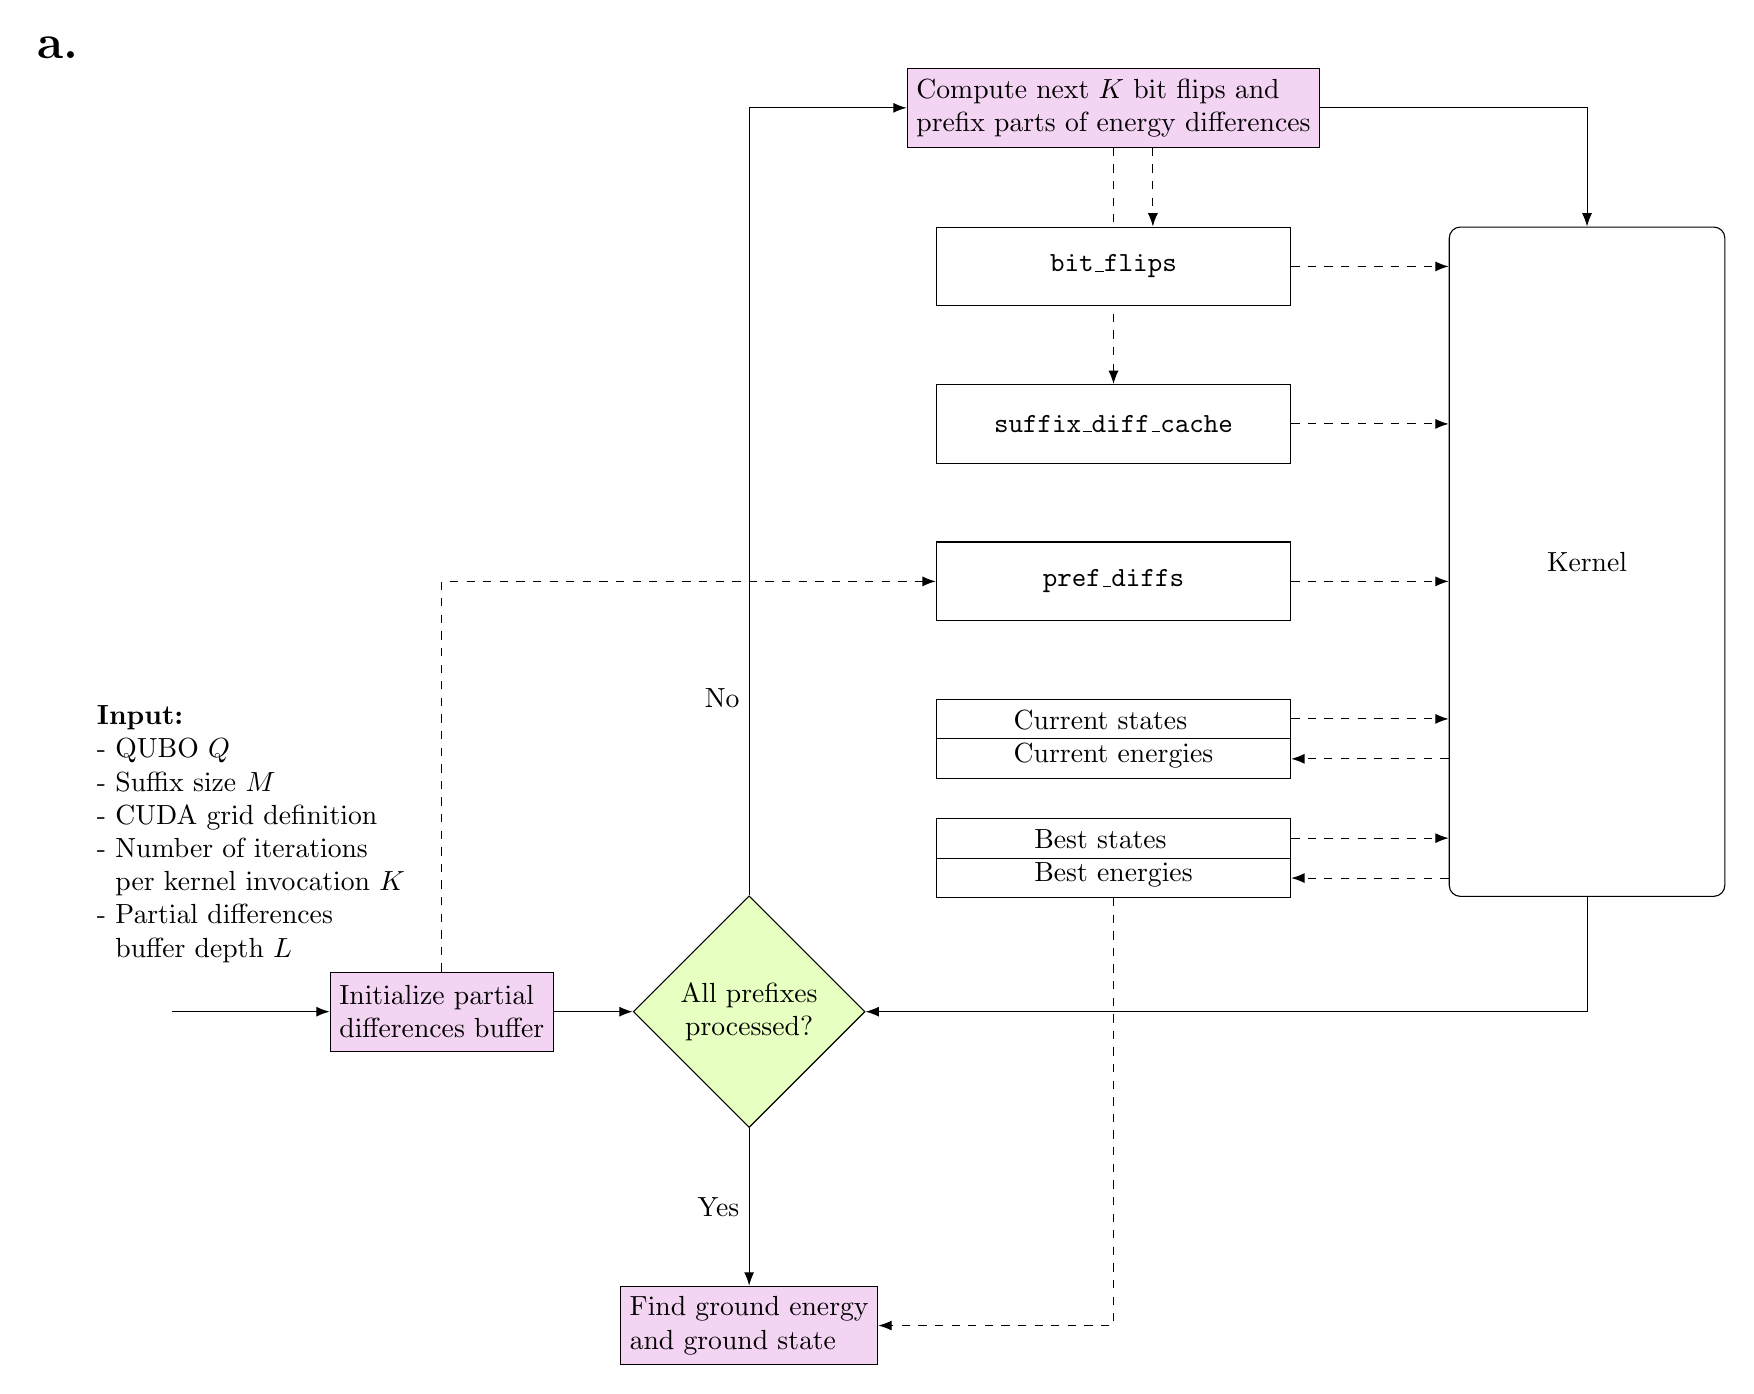
\begin{tikzpicture}[
    memcell/.style={draw, rectangle, minimum width=0.2cm, minimum height=0.2cm},
    memarray/.style={minimum width=4.5cm, fill=white,minimum height=1cm, draw},
    energies/.style={memarray, nodes={memcell, fill=Energies}},
    rect/.style={minimum height=1cm, fill=Rect, draw, rectangle, align=left},
    decision/.style={draw, align=center, diamond, fill=Decision},
    every node/.style={font={\normalsize}},
    brace/.style={decorate,decoration={brace,amplitude=5pt,mirror,raise=1mm}},
    brace2/.style={decorate,decoration={brace,amplitude=5pt,mirror,raise=4mm}},
    subroutine/.style={draw, rounded corners},
    subsubroutine/.style={subroutine,dashed,thick},
    gpuio/.style={-Latex,dashed},
    baseline=(a)
  ]

  \node(start) {};

  \node[rect, right=2cm of start] (initialize) {
    Initialize partial\\differences buffer
  };

  \node[decision, right=1cm of initialize] (decision)
  {All prefixes\\processed?};

  \coordinate [above=10cm of decision] (c1);

  \node[rect, right=2cm of c1] (prefix) {Compute next $K$ bit flips and\\prefix parts of energy differences};

  \node[memarray, below=3cm of prefix] (prediffs) {\texttt{suffix\_diff\_cache}};
  \draw[gpuio] (prefix) -- (prediffs);
  \node[memarray, below=1cm of prefix] (flips) {\texttt{bit\_flips}};
  \draw[gpuio] ($(prefix.south)+(0.5cm,0)$) -- ($(flips.north)+(0.5cm,0)$);
  \node[memarray, below=5cm of prefix] (pdiffs) {\texttt{pref\_diffs}};

  \node[memarray, below=7cm of prefix, align=left] (current) {Current states\\Current energies};
  \draw (current.east) -- (current.west);

  \node[memarray, below=0.5cm of current, align=left] (best) {Best states\\Best energies};
  \draw (best.east) -- (best.west);

  \coordinate[right=3cm of prefix] (c2);

  \node[
    subroutine,
    minimum width=3.5cm,
    minimum height=8.5cm,
    right=2cm of flips.north east,
    anchor=north west
  ]
  (kernel)
  {Kernel};

  \node[rect, below=2cm of decision] (output) {Find ground energy\\and ground state};


  \draw[gpuio] (flips.east) -- (flips-|kernel.south west);
  \draw[gpuio] (prediffs.east) -- (prediffs-|kernel.south west);
  \draw[gpuio] (pdiffs.east) -- (pdiffs-|kernel.south west);
  \coordinate (c3) at ($(current.east)!0.5!(current.north east)$);
  \coordinate (c4) at ($(current.east)!0.5!(current.south east)$);

  \coordinate (c5) at ($(best.east)!0.5!(best.north east)$);
  \coordinate (c6) at ($(best.east)!0.5!(best.south east)$);

  \draw[gpuio] (c3) -- (c3-|kernel.south west);
  \draw[gpuio] (c4-|kernel.south west) -- (c4);

  \draw[gpuio] (c5) -- (c5-|kernel.south west);
  \draw[gpuio] (c6-|kernel.south west) -- (c6);

  \draw[-Latex] (start) -- (initialize)
  node[midway, above=0.5, align=left]
  {
    \textbf{Input:}\\
    - QUBO $Q$\\
    - Suffix size $M$\\
    - CUDA grid definition\\
    - Number of iterations \\
      ~~per kernel invocation $K$\\
    - Partial differences\\
      ~~buffer depth $L$
  };

  \draw[-Latex] (initialize) -- (decision);
  \draw (decision) -- (c1) node[near start, left] {No};
  \draw[-Latex] (c1) -- (prefix);
  \draw[gpuio] (initialize) |- (pdiffs);
  \draw[-Latex] (kernel) |- (decision);
  \draw[gpuio] (best) |- (output);
  \draw[-Latex] (decision) -- (output) node[midway, left] {Yes};
  \draw[-Latex] (prefix) -| (kernel.north);

  \node at (current bounding box.north west) [anchor=south east] (a) {\LARGE \textbf{a.}};
\end{tikzpicture}
\end{document}
